

\newcommand{\dmsimp}{\textsc{DMsimp}\xspace}
\newcommand{\maddm}{\textsc{MadDM}\xspace}


\section{Relic Density}

%CD: not sure we need the sentence below
%The relic density observed today critically depends on the interactions between SM and DM particles in the early universe. When the temperature of the universe is sufficiently large, the rate of mediated interactions can be large and DM coexists with matter. As the universe cools off, the rate of interactions between the dark and visible sectors will be reduced, leaving residual DM and matter. For cases where the interaction between the sectors is strong, DM will readily decay into matter, thus reducing the overall DM abundance. For cases where the interaction is weak, it will freeze out at an earlier time scale (corresponding to a higher temperature scale) and the resulting DM density will be larger. 

DM simplified models used for searches at collider experiments can be used to predict the DM relic density in the universe under the following assumptions: 

\begin{itemize}
\item DM only couples to SM matter only through the one mediator explicitly included in the model.
\item No additional undiscovered particles couple to the mediator.
\item No additional mechanisms exist to generate DM.
\end{itemize}

Generally, it should also be noted that simplified models are not full theories. Since the evolution of the universe probes all energy scales, additional degrees of freedom at higher energy scales that would not necessarily modify collider signatures may significantly alter the relic density.

Under these conditions, the relic density obtained using the model can be compared with measurements such as the most recent results by the Planck collaboration~\cite{Planck} to gain insight on the viability of a given choice of model parameters.

In this section, we present an analytical calculation of the relic density for the most relevant processes. We then compute the relic density for the vector, axial-vector, scalar, and pseudo-scalar coupling scenarios following the Langrangian definition specified in LHC DM working group document~\cite{Boveia:2016mrp} using the program \maddm~\cite{Backovic:2013dpa,Backovic:2015tpt}. The coupling values used for this section are representative. The coupling to SM quarks of spin-1 mediators (vector and axial-vector) is chosen to be $g_{\rm q} = 0.25$ and the lepton coupling is set to zero, corresponding to case V1 and A1 of Sec.~\ref{sub:vecAxial}. For spin-0 mediators (scalar and pseudo-scalar), the coupling to quarks is chosen to be $g_{\rm q}=1.0$ with an implicit Yukawa scaling for all SM particles. For both models, the coupling between the mediator and the DM is fixed to be $g_{\rm DM}=1$, without Yukawa scaling. These couplings are only used for display purposes in this document, and the full set of relic density curves can be found on the DMWG SVN repository~\cite{SVNRepo}. 

\subsection{Analytical expression for the DM relic density}

\begin{center}
\begin{figure}[!h]
\centering
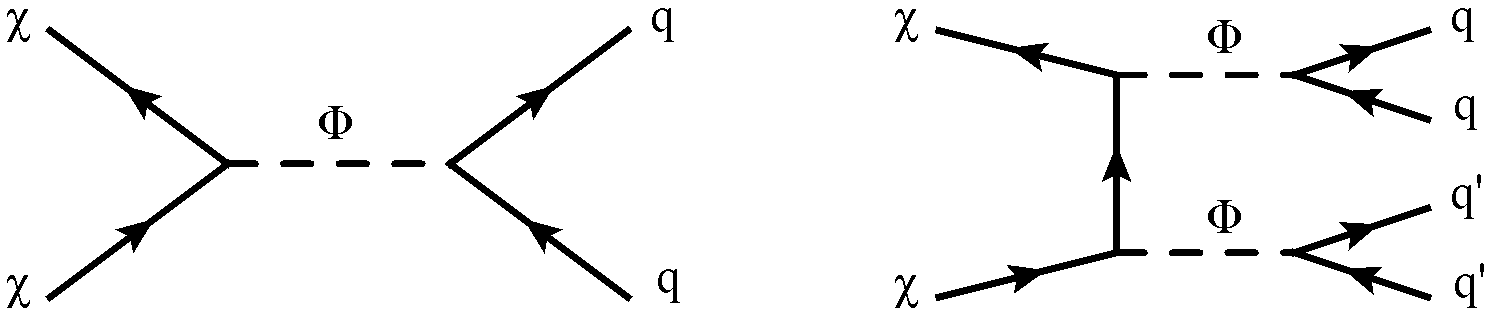
\includegraphics[width=0.78\textwidth]{figures/DMAnnihilationDiagrams.png} 
\caption{Feynman graphs of s-channel (left) and t-channel (right) DM annihilation. While the s-channel process is dominant for $m_{\rm med}/2 > m_{\rm DM}$, the region $m_{\rm med} < m_{\rm DM}$ is dominated by the t-channel diagram.}
\label{fig:relicprod}
\end{figure}
\end{center}

The s-channel production of a single mediator and t-channel production of a mediator pair in Fig.~\ref{fig:relicprod} are the two main interaction relevant for the calculation of the relic density.
For $m_{\rm med} > m_{\rm DM}$, the s-channel process dominates, while the t-channel process gives the main contribution for $m_{\rm med} < m_{\rm DM}$.

Analytic forms for the relic density $\Omega h^{2}$ can be derived separately for both processes. 
The relic density for the s-channel process for scalar and vector mediator scenarios are given in Eqn.~\ref{eq:SS} and~\ref{eq:SV}.

%\begin{equation}
%\label{eq:SS}
%    \Omega h^{2}  \propto  \left[\Sigma_{q} \frac{g_{\rm DM}^2 g_{\rm q}^2 y_{q}^2}{32\pi s } %\frac{\left(s-4m^2_{q}\right)^{3/2}\sqrt{s-4m_{\rm DM}^2}}{\left(s-m_{\rm med}^2\right)^2} \right]^{-1} \
%\end{equation}
%\begin{equation}
%\label{eq:SV}
%\Omega h^{2} & \propto & \left[\Sigma_{q} \frac{g_{\rm DM}^2 g_{\rm q}^2           }{32\pi s } %\frac{\left(s-4m^2_{q}\right)^{3/2}        (s+2m_{\rm DM}^2)}{\left(s-m_{\rm med}^2\right)^2\sqrt{s-4m_{\rm DM}^2}} \right]^{-1}
%\end{equation}

\begin{eqnarray}
\label{eq:SS} \Omega h^{2} & \propto & \left[\Sigma_{q} \frac{g_{\rm DM}^2 g_{\rm q}^2 y_{q}^2}{32\pi s } \frac{\left(s-4m^2_{q}\right)^{3/2}\sqrt{s-4m_{\rm DM}^2}}{\left(s-m_{\rm med}^2\right)^2} \right]^{-1} \\
\label{eq:SV} \Omega h^{2} & \propto & \left[\Sigma_{q} \frac{g_{\rm DM}^2 g_{\rm q}^2           }{32\pi s } \frac{\left(s-4m^2_{q}\right)^{3/2}        (s+2m_{\rm DM}^2)}{\left(s-m_{\rm med}^2\right)^2\sqrt{s-4m_{\rm DM}^2}} \right]^{-1}. 
\end{eqnarray}

Summation over the quark index q is implied. The Yukawa coupling modifier is denoted as $y_{q}$ and the masses of mediator and DM particle are referred to as $m_{\rm med}$ and $m_{\rm DM}$, respectively. Finally, $s$ denotes the center of mass energy which is varied in the thermalization process. 
%CD: removed, what does this mean?
%In this analytic expression, the reciprocal relationship between the relic density and coupling parameters is evident. 

Similarly, one can derive the relic density expression for
%CD: not sure closed form is something that we want to use here?
%a closed form 
for the t-channel interaction, where~\ref{eq:TS} represents the scalar and~\ref{eq:TV} the axial-vector scenario:

%\begin{equation}
%\label{eq:TS}
%\Omega h^2  \propto  \left g_{\rm DM}^4\frac{m_{\rm DM}\sqrt{m_{\rm DM}^2-m_{\rm med}^2}( 9m_{\rm DM}^4+8m_{\rm DM}^2m_{\rm med}^2+2m_{\rm med}^4)}{3\pi\left(m_{\rm med}^2-2m_{\rm DM}^2\right)^4} \right]^{-1}
%\end{equation}

%\begin{equation}
%\label{eq:TV}
%\Omega h^2  \propto  FORMULA 
%\end{equation}

\begin{eqnarray}
\label{eq:TS} \Omega h^2 & \propto & \left[g_{\rm DM}^4\frac{m_{\rm DM}\sqrt{m_{\rm DM}^2-m_{\rm med}^2}( 9m_{\rm DM}^4+8m_{\rm DM}^2m_{\rm med}^2+2m_{\rm med}^4)}{3\pi\left(m_{\rm med}^2-2m_{\rm DM}^2\right)^4} \right]^{-1} \\  
\label{eq:TV} \Omega h^2 & \propto & \left[\frac{ (g_{\rm DM})^4 (m_{\rm DM}^2 - m_{\rm med}^2)^{3/2}}{4 \pi \, m_{\rm DM}(m_{\rm med}^2 - 2 m_{\rm DM}^2)^2}  \right]^{-1}     
\end{eqnarray}

%{\bf OB: Need to add formula for~\label{eq:TV}}
%PT: I have added this formula. It is correct under the assumptions I've added towards the end

\subsection{Numerical results}

The numerical calculation of the relic density is performed using the program \maddm~\cite{Backovic:2013dpa,Backovic:2015tpt}. \maddm considers all tree-level $2\rightarrow2$ interaction modes between DM and SM particles. The processes are thermalized and the resulting relic density is computed.
For this result, we use version 2.0 of the \dmsimp implementation of the simplified model scenarios~\cite{Backovic:2015soa,Neubert:2015fka,Mattelaer:2015haa} and \maddm version 2.0.6.
Since \maddm does not yet support on-the-fly calculation of the mediator width from the model parameters, the \dmsimp model was manually modified to use the mediator width formulas given in Ref.~\cite{Boveia:2016mrp}. The calculation provided in the previous DMWG recommendations~\cite{Pree:2016hwc} used a previous version of \maddm, which did not include the t-channel process. 

%ABCD: Below not significant because they've been tested 
%Less significantly, since the \dmsimp implementation was not available at the time, the results were derived using a previous implementation of  simplified models, which are however equivalent to the \dmsimp models in physics content.

Figures~\ref{fig:DMBounds} and~\ref{fig:DMBoundsg1} show the DM relic density in the $m_{\rm med}$-$m_{\rm DM}$ plane for the benchmark scalar, pseudo-scalar, vector, and axial-vector coupling scenarios. In all cases, solid contours correspond to the parameters where the correct DM relic abundance is obtained from standard thermal freeze-out for the chosen couplings. Regions where the relic density is either higher or lower than the observed value are referred to as over- and underabundance regions, respectively.

In all coupling scenarios, overabundance of DM is observed for $m_{\rm DM}<m_{\rm med}$. While the exact characteristics of this region depend on the coupling scenario, its size is generally anti-correlated with the coupling strength $g_{\rm q}$. For larger couplings, the DM particles can more easily annihilate into SM particles, which reduces the relic density and thus the size of the overabundance regions.

For the vector coupling scenario, no features beyond the generic overabundance region are observed. This case is fully consistent with previous results.

In the scenario of axial-vector coupling, the generic overabundance region extends to higher $m_{\rm DM}$ than in the vector case. Additionally, there is an overabundance region above the diagonal $m_{\rm DM}=m_{\rm med}/2$. While this region is also present in the previous results, its width in mediator mass is significantly narrower, due to the relevance of the t-channel process for $m_{\rm DM}>m_{\rm med}$. 

For a mediator with scalar couplings, the overabundance region for small $m_{\rm DM}$ is bounded by the top-threshold $m_{\rm DM}\approx m_{\rm top}$, above which annihilation into top quark pairs is allowed. Additional overabundance regions are observed for $m_{\rm med} > m_{\rm DM} > m_{\rm med}/2$, where the upper bound is due to the onset of mediator pair production and the lower bound reflects the resonant enhancement of DM annihilation to SM particle pairs. The inclusion of the t-channel process induces a significant reduction in the relic density for $m_{\rm med} > m_{\rm DM}$, which was previously over- and is now underabundant.

The pseudo-scalar case is generally similar to the scalar scenario, with the regions of overabundance being less pronounced due to the increased annihilation cross-section. Consequently, no regions of overabundance are observed above the top threshold and the triangular region at $m_{\rm DM} > m_{\rm med}/2$ is reduced in size. While the strong reduction of the relic density above the top threshold is fully consistent with the previous results, again, a new threshold is introduced at $m_{\rm DM} \approx m_{\rm med}$.

\begin{center}
\begin{figure}[h]
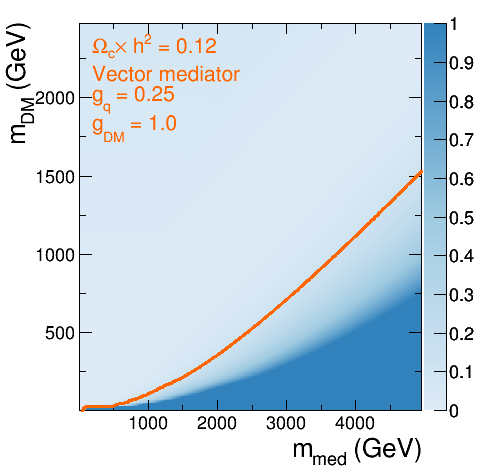
\includegraphics[width=0.49\textwidth]{figures/scan_V_g25_MD_xxd_V_gq25.png} 
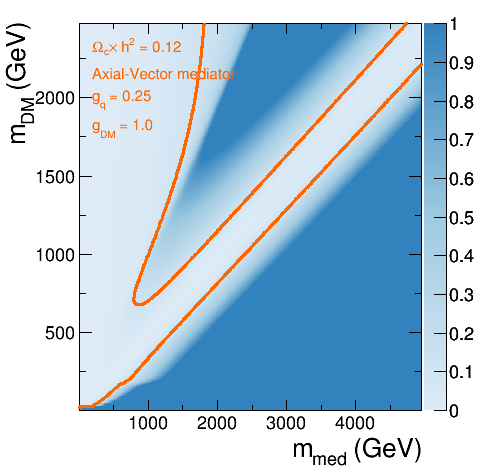
\includegraphics[width=0.49\textwidth]{figures/scan_A_g25_MD_xxd_A_gq25.png} \\
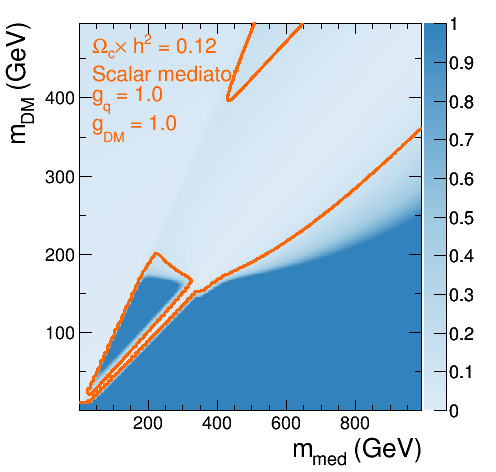
\includegraphics[width=0.49\textwidth]{figures/scan_S_g1_MD_xxd_S_gq1.png} 
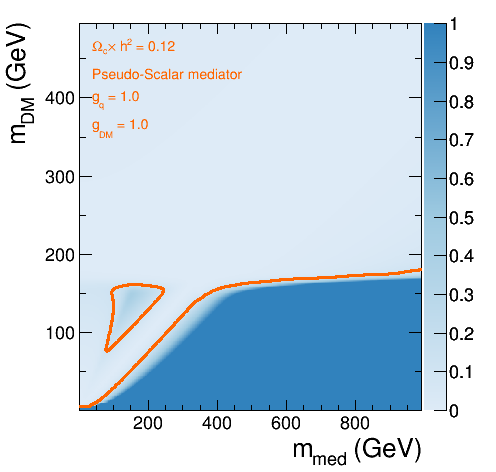
\includegraphics[width=0.49\textwidth]{figures/scan_P_g1_MD_xxd_P_gq1.png} \\
\caption{The predicted relic density $\Omega h^{2}$ in the $m_{\rm med}$-$m_{\rm DM}$ plane for a vector (top-left) and axial-vector mediator (top-right), both with couplings $g_{\rm q}=0.25$ and $g_{\rm DM}=1.0$, and for a scalar (bottom left) and pseudo-scalar mediator (bottom right) with couplings $g_{\rm q}=g_{\rm DM}=1.0$.
The contour lines correspond to the region of parameter space where the relic density is consistent with the value $\Omega h^2=0.1185 \pm 0.0020$, as measured by the Planck collaboration. The impact of the uncertainty on the position of the contours is consistent with the line width.}
\label{fig:DMBounds}
\end{figure}
\end{center}

\begin{center}
\begin{figure}[h]
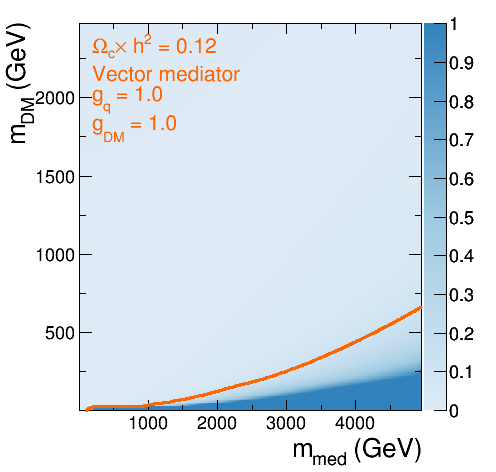
\includegraphics[width=0.49\textwidth]{figures/scan_V_g1_MD_xxd_V_gq1.png} 
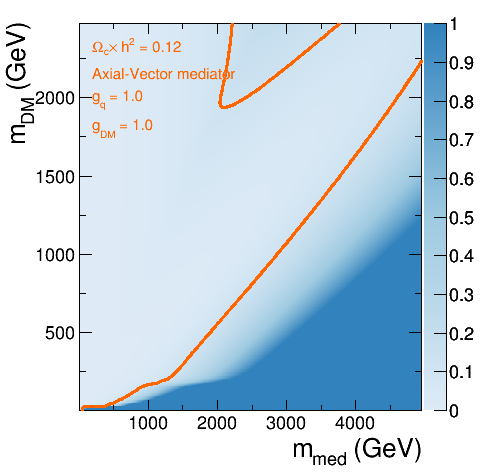
\includegraphics[width=0.49\textwidth]{figures/scan_A_g1_MD_xxd_A_gq1.png} \\
\caption{The predicted relic density $\Omega h^{2}$ in the $m_{\rm med}$-$m_{\rm DM}$ plane for a vector (left) and axial-vector mediator (right), both with couplings $g_{\rm q}=1$ and $g_{\rm DM}=1$.}
\label{fig:DMBoundsg1}
\end{figure}
\end{center}


\subsection{Comparison of analytical results to full calculation}

\begin{center}
\begin{figure}[h]
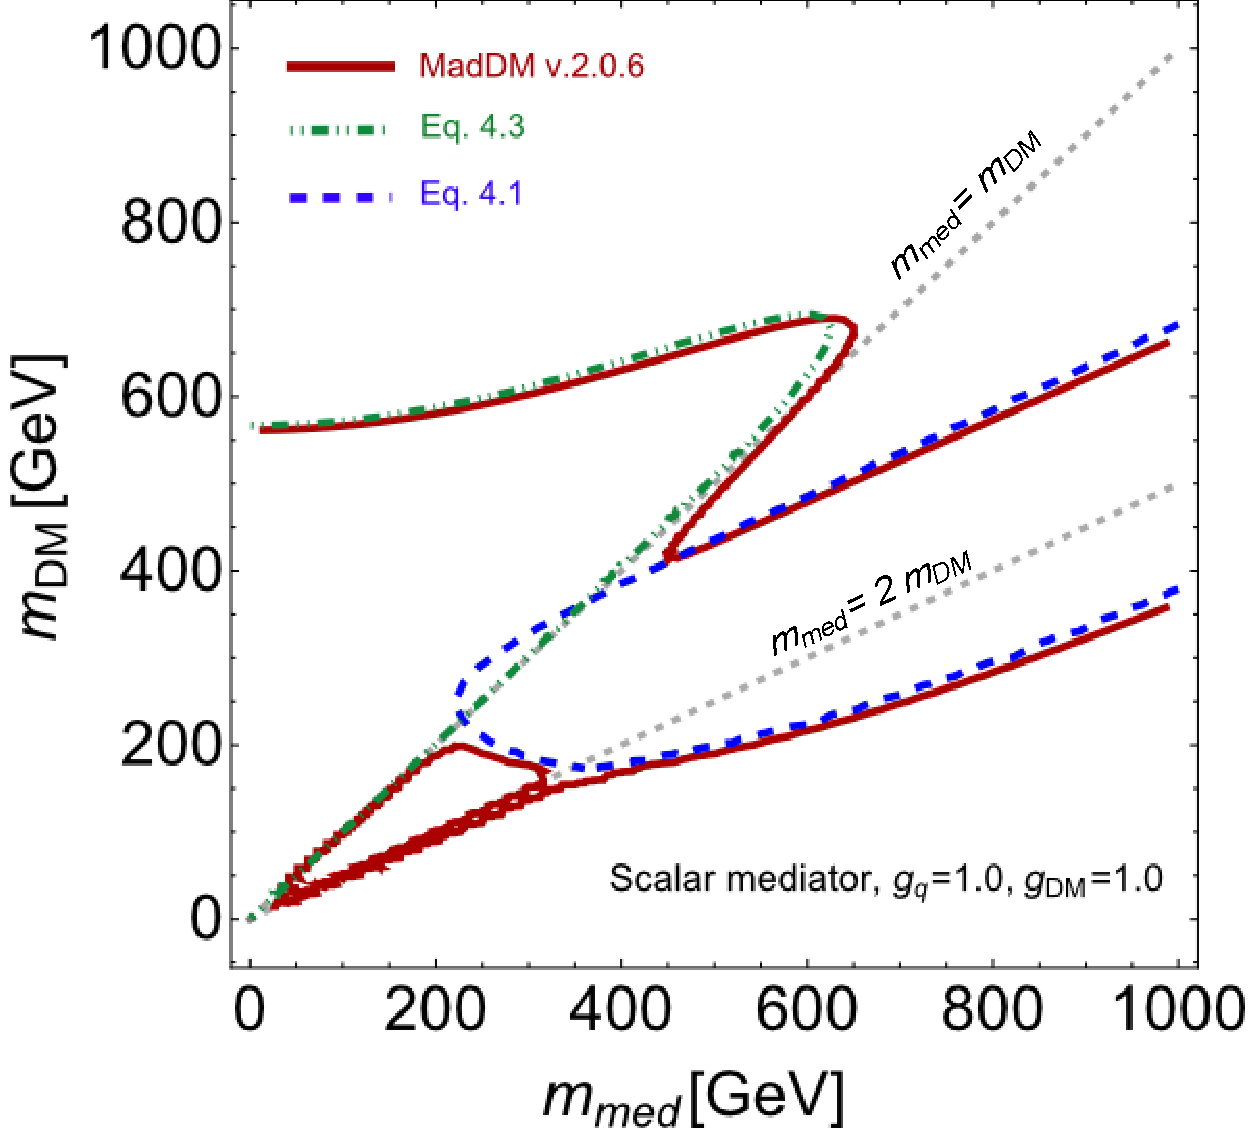
\includegraphics[width=0.49\textwidth]{figures/scalar_mediator_omegah2.pdf}
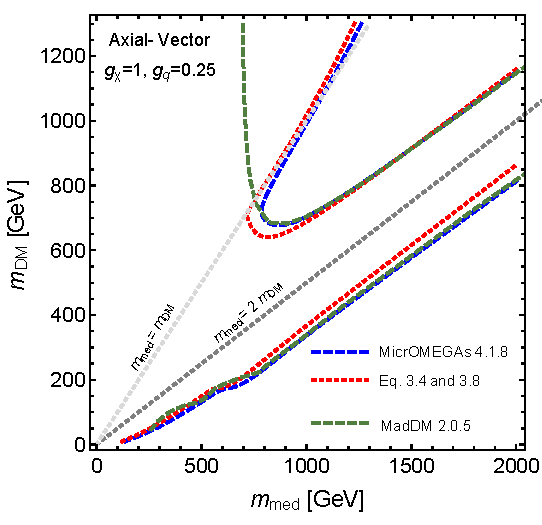
\includegraphics[width=0.49\textwidth]{figures/AV_comparison2.pdf} 
\caption{Comparison of the analytic calculation of the relic density with numerical results from \maddm and for scalar (left) and axial-vector couplings (right). In the case of the axial-vector coupling, \maddm v 2.0.5 is used as representative of previous results without the t-channel process, while the \textsc{MicrOMEGAs} output agrees with \maddm.}
\label{fig:analcalc}
\end{figure}
\end{center}

In figure~\ref{fig:analcalc} we compare the analytical results of the two production modes with the full calculation performed in \maddm and \textsc{MicrOMEGAs}.
To obtain the analytical curves precisely the cross section should be thermally averaged and the freeze-out temperature should be determined numerically. However one can obtain good agreement by estimating the ratio of the DM mass to freeze-out temperature as was done in figure~\ref{fig:analcalc} for the axial vector where we assumed this ratio to be 28 across the parameter space, and similarly estimated the effective number of relativistic degrees of freedom. We expanded the cross section in powers of the DM velocity which is not exact and care should be taken with this approach since it can break down in certain regimes, for example on resonance~\cite{Gondolo:1990dk}
%PT: this is the text I've added
For the limiting cases where one of the interactions dominates, the analytic solutions and full numerical calculation are in good agreement. 





